\documentclass[12pt,a4paper]{article}
\usepackage[utf8]{inputenc}
\usepackage[margin=1in]{geometry}
\usepackage{graphicx}
\usepackage{listings}
\usepackage{xcolor}
\usepackage{hyperref}
\usepackage{fancyhdr}
\usepackage{tikz}
\usepackage{longtable}
\usepackage{array}
\usetikzlibrary{shapes.geometric, arrows}

\hypersetup{
    colorlinks=true,
    linkcolor=blue,
    urlcolor=blue
}

\lstdefinestyle{codeblock}{
    backgroundcolor=\color{gray!10},
    basicstyle=\ttfamily\footnotesize,
    breaklines=true,
    captionpos=b,
    commentstyle=\color{green!50!black},
    keywordstyle=\color{blue!80!black},
    stringstyle=\color{red!60!black},
    numbers=left,
    numberstyle=\tiny\color{gray},
    numbersep=5pt,
    showstringspaces=false,
    frame=single,
    rulecolor=\color{gray!40}
}

\lstset{style=codeblock}

\pagestyle{fancy}
\fancyhf{}
\lhead{Web Lab Report}
\rhead{Django Concepts Lab}
\rfoot{Page \thepage}

\tikzstyle{startstop} = [rectangle, rounded corners, minimum width=2.8cm, minimum height=1cm, text centered, draw=black, fill=red!20, font=\small]
\tikzstyle{process} = [rectangle, minimum width=3.4cm, minimum height=1cm, text centered, text width=3.4cm, draw=black, fill=blue!15, font=\small]
\tikzstyle{decision} = [diamond, minimum width=2.8cm, minimum height=1cm, text centered, draw=black, fill=green!20, aspect=2.4, font=\small]
\tikzstyle{arrow} = [thick,->,>=stealth]

\title{\textbf{Web Technology Lab Report}\\Django Concepts Demonstration Application}
\author{Student Name: Chandan Kumar Shah\\Roll Number: 080BCT023}

\begin{document}

\begin{titlepage}
    \centering
    \vspace*{1cm}

    {\Large \textbf{TRIBHUVAN UNIVERSITY}}\\
    \vspace{0.3cm}
    {\Large \textbf{INSTITUTE OF ENGINEERING}}\\
    \vspace{0.3cm}
    {\Large \textbf{PULCHOWK CAMPUS}}\\

    \vspace{1.4cm}

    
\includegraphics[width=5.5cm]{emblem.png}\\

    \vspace{1.5cm}

    {\Huge \textbf{LAB REPORT}}\\
    \vspace{0.4cm}
    {\Large \textbf{Web Technology Lab Assignment}}\\
    \vspace{0.3cm}
    {\Large \textbf{Django Concepts Demonstration Application}}\\

    \vspace{0.9cm}
    {\large \textbf{GitHub Repository}}\\
    {\normalsize \url{https://github.com/chandan11248/libraryhub-django-portal}}\\

    \vspace{2cm}

    \begin{minipage}{0.45\textwidth}
        \begin{flushleft} \large
            \textbf{Submitted by:}\\
            Name: Chandan Kumar Shah\\
            Roll No: 080BCT023\\
            Department: Electronics and\\
            Computer Engineering
        \end{flushleft}
    \end{minipage}
    \hfill
    \begin{minipage}{0.45\textwidth}
        \begin{flushright} \large
            \textbf{Submitted to:}\\
            Department of Electronics\\
            and Computer Engineering
        \end{flushright}
    \end{minipage}

    \vfill
\end{titlepage}

\tableofcontents
\newpage

\section{Brief Description of the Project}
This project is a Django-based web application named \textbf{LibraryHub Django Portal}, developed to illustrate important web development concepts such as request and response handling, form processing, sessions, URL routing, custom middleware, templating, database integration, authentication, authorization, and CRUD operations.

The system allows users to browse books, search by title or category, register and log in, borrow and return books, manage categories, and view recent activity logs. It uses Django's ORM with SQLite as the relational database and demonstrates clean separation of concerns through Django's MVT architecture.

\section{Concepts Illustrated by the Project}
\begin{itemize}
    \item \textbf{Handling Requests \& Responses:} Views such as \texttt{home}, \texttt{book\_list}, and \texttt{api\_books} handle GET requests, return HTML responses, and return JSON responses.
    \item \textbf{Form Data Handling \& Sessions:} Django forms are used for books, categories, registration, and search. Sessions are used for visit count, borrowed books, and remember-me login behavior.
    \item \textbf{Routing, Middleware, Templating:} URL patterns in \texttt{library/urls.py} route requests to views. Custom middleware handles logging, security, error reporting, and session tracking. Templates are used to render the user interface.
    \item \textbf{Database Integration:} The system uses SQLite as a relational database. Models such as \texttt{Book}, \texttt{Category}, and \texttt{BorrowRecord} demonstrate CRUD operations and ORM relationships.
    \item \textbf{Relational vs NoSQL:} This project uses a relational database because book, category, and borrow relationships are structured and well-suited to foreign keys. In a NoSQL system, the same data could be stored as documents, but relationship queries would be less normalized.
    \item \textbf{Authentication \& Authorization:} Django authentication is used for registration, login, logout, session cookies, and protecting selected views with \texttt{@login\_required}.
    \item \textbf{Middleware for Logging, Error Handling, and Security:} Custom middleware logs each request, adds security headers, blocks suspicious requests, handles exceptions, and tracks visit counts in sessions.
\end{itemize}

\section{MVT Architecture of the Project}
Django follows the MVT (Model-View-Template) architecture.

\subsection{Model}
The models define the database structure and business relationships.
\begin{itemize}
    \item \texttt{Category}
    \item \texttt{Book}
    \item \texttt{BorrowRecord}
    \item \texttt{ActivityLog}
\end{itemize}

\subsection{View}
The views receive requests, process logic, query the database, and return responses.
\begin{itemize}
    \item \texttt{home}
    \item \texttt{book\_list}
    \item \texttt{book\_create}, \texttt{book\_update}, \texttt{book\_delete}
    \item \texttt{register\_view}, \texttt{login\_view}, \texttt{logout\_view}
    \item \texttt{api\_books}
\end{itemize}

\subsection{Template}
Templates define the presentation layer for HTML pages.
\begin{itemize}
    \item \texttt{base.html}
    \item \texttt{home.html}
    \item \texttt{book\_list.html}
    \item \texttt{book\_detail.html}
    \item \texttt{login.html}, \texttt{register.html}
\end{itemize}

\subsection{MVT Architecture Diagram}
\begin{center}
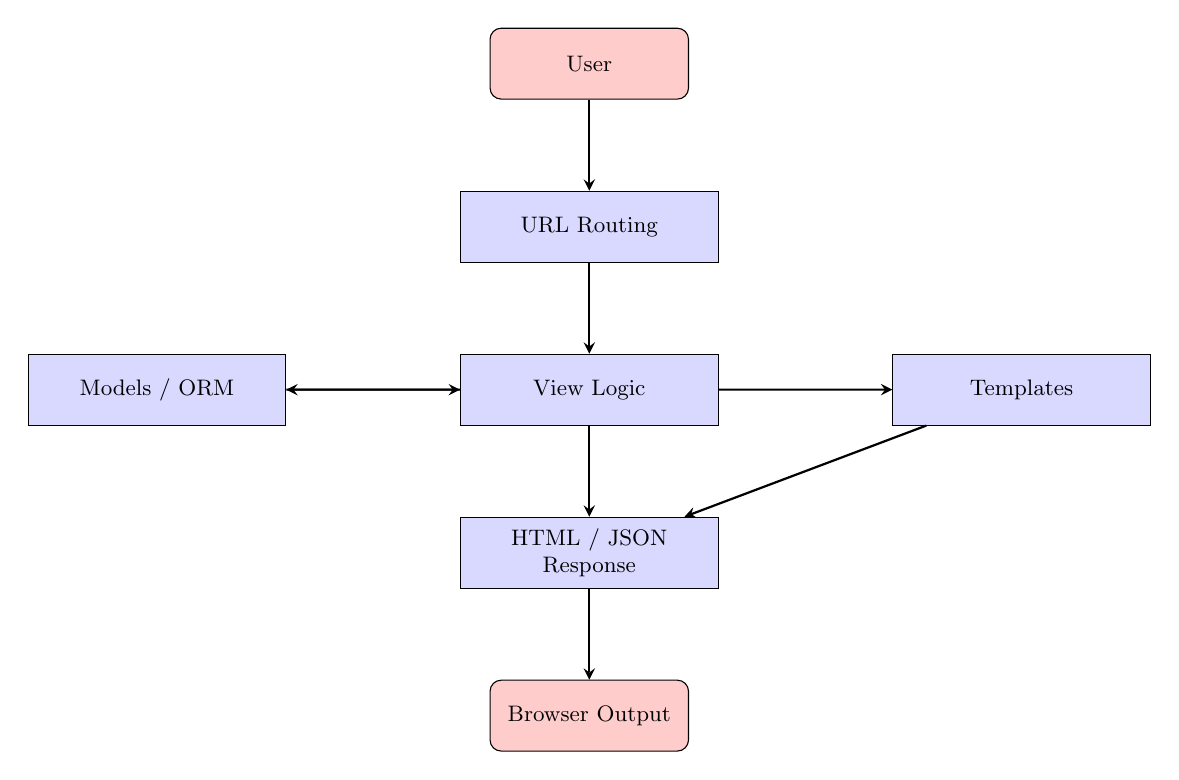
\begin{tikzpicture}[node distance=2.3cm, scale=0.9, transform shape]
\node (user) [startstop] {User};
\node (url) [process, below of=user] {URL Routing};
\node (view) [process, below of=url] {View Logic};
\node (model) [process, left of=view, xshift=-3.8cm] {Models / ORM};
\node (template) [process, right of=view, xshift=3.8cm] {Templates};
\node (response) [process, below of=view] {HTML / JSON Response};
\node (end) [startstop, below of=response] {Browser Output};

\draw [arrow] (user) -- (url);
\draw [arrow] (url) -- (view);
\draw [arrow] (view) -- (model);
\draw [arrow] (model) -- (view);
\draw [arrow] (view) -- (template);
\draw [arrow] (template) -- (response);
\draw [arrow] (view) -- (response);
\draw [arrow] (response) -- (end);
\end{tikzpicture}
\end{center}

\section{Project Structure}
\begin{lstlisting}[caption=Project Directory Structure]
Lab-4/
|-- library/
|   |-- models.py
|   |-- views.py
|   |-- urls.py
|   |-- forms.py
|   |-- middleware.py
|   `-- templates/library/
|-- library_project/
|   |-- settings.py
|   `-- urls.py
|-- manage.py
|-- requirements.txt
`-- screenshot.png
\end{lstlisting}

\section{Major Components of the Project}

\subsection{Models}
The models define relational database entities and ORM relationships.

\begin{lstlisting}[language=Python, caption=Major Models]
from django.db import models
from django.contrib.auth.models import User


class Category(models.Model):
    name = models.CharField(max_length=100, unique=True)
    description = models.TextField(blank=True)


class Book(models.Model):
    title = models.CharField(max_length=200)
    author = models.CharField(max_length=150)
    isbn = models.CharField(max_length=13, unique=True)
    category = models.ForeignKey(Category, on_delete=models.CASCADE, related_name='books')
    published_date = models.DateField()
    copies_available = models.PositiveIntegerField(default=1)


class BorrowRecord(models.Model):
    user = models.ForeignKey(User, on_delete=models.CASCADE, related_name='borrow_records')
    book = models.ForeignKey(Book, on_delete=models.CASCADE, related_name='borrow_records')
    status = models.CharField(max_length=10, default='borrowed')
\end{lstlisting}

\subsection{URLs}
The URL configuration maps browser requests to the proper Django views.

\begin{lstlisting}[language=Python, caption=library/urls.py]
from django.urls import path
from . import views

urlpatterns = [
    path('', views.home, name='home'),
    path('books/', views.book_list, name='book_list'),
    path('books/<int:pk>/', views.book_detail, name='book_detail'),
    path('books/add/', views.book_create, name='book_create'),
    path('books/<int:pk>/edit/', views.book_update, name='book_update'),
    path('books/<int:pk>/delete/', views.book_delete, name='book_delete'),
    path('register/', views.register_view, name='register'),
    path('login/', views.login_view, name='login'),
    path('logout/', views.logout_view, name='logout'),
    path('api/books/', views.api_books, name='api_books'),
]
\end{lstlisting}

\subsection{Forms}
Forms are used for safe form handling and validation.

\begin{lstlisting}[language=Python, caption=Form Components]
class BookForm(forms.ModelForm):
    class Meta:
        model = Book
        fields = ['title', 'author', 'isbn', 'category', 'published_date',
                  'copies_available', 'description']


class UserRegistrationForm(UserCreationForm):
    email = forms.EmailField(required=True)


class SearchForm(forms.Form):
    query = forms.CharField(max_length=200, required=False)
    category = forms.ModelChoiceField(queryset=Category.objects.all(), required=False)
\end{lstlisting}

\subsection{Views}
The views demonstrate request handling, response generation, CRUD, authentication, and JSON output.

\begin{lstlisting}[language=Python, caption=View Components]
def home(request):
    books = Book.objects.select_related('category').all()[:6]
    return render(request, 'library/home.html', context)


@login_required
def book_create(request):
    if request.method == 'POST':
        form = BookForm(request.POST)
        if form.is_valid():
            form.save()
            return redirect('book_list')
    else:
        form = BookForm()
    return render(request, 'library/book_form.html', {'form': form})


def api_books(request):
    books = Book.objects.select_related('category').all()
    return JsonResponse(data)
\end{lstlisting}

\subsection{Middleware}
Custom middleware is one of the main strengths of this project.

\begin{lstlisting}[language=Python, caption=Custom Middleware]
class RequestLoggingMiddleware(MiddlewareMixin):
    def process_request(self, request):
        request._start_time = time.time()

    def process_response(self, request, response):
        return response


class SecurityMiddleware(MiddlewareMixin):
    def process_request(self, request):
        return None

    def process_response(self, request, response):
        response['X-Content-Type-Options'] = 'nosniff'
        return response


class VisitCounterMiddleware(MiddlewareMixin):
    def process_request(self, request):
        if not request.session.get('visit_count'):
            request.session['visit_count'] = 0
        request.session['visit_count'] += 1
\end{lstlisting}

\subsection{Settings}
The settings file shows session configuration, middleware registration, app registration, and database settings.

\begin{lstlisting}[language=Python, caption=Important settings.py Sections]
INSTALLED_APPS = [
    'django.contrib.admin',
    'django.contrib.auth',
    'django.contrib.contenttypes',
    'django.contrib.sessions',
    'django.contrib.messages',
    'django.contrib.staticfiles',
    'library',
]

MIDDLEWARE = [
    'django.middleware.security.SecurityMiddleware',
    'django.contrib.sessions.middleware.SessionMiddleware',
    'django.middleware.common.CommonMiddleware',
    'django.contrib.auth.middleware.AuthenticationMiddleware',
    'library.middleware.RequestLoggingMiddleware',
    'library.middleware.SecurityMiddleware',
    'library.middleware.ErrorHandlingMiddleware',
    'library.middleware.VisitCounterMiddleware',
]

DATABASES = {
    'default': {
        'ENGINE': 'django.db.backends.sqlite3',
        'NAME': BASE_DIR / 'db.sqlite3',
    }
}
\end{lstlisting}

\section{CRUD Operations in the Project}
The CRUD operations are implemented mainly for the \texttt{Book} model:
\begin{itemize}
    \item \textbf{Create:} \texttt{book\_create}
    \item \textbf{Read:} \texttt{book\_list} and \texttt{book\_detail}
    \item \textbf{Update:} \texttt{book\_update}
    \item \textbf{Delete:} \texttt{book\_delete}
\end{itemize}

These operations are implemented through Django forms, model queries, and template rendering.

\section{Database Integration: Relational vs NoSQL}
This project uses SQLite, which is a relational database. The relational approach is useful here because the project contains well-defined structured relationships:
\begin{itemize}
    \item a \texttt{Book} belongs to one \texttt{Category},
    \item a \texttt{BorrowRecord} connects a \texttt{User} and a \texttt{Book},
    \item activity logs are stored as structured records.
\end{itemize}

Django's ORM makes relational database access easier by allowing database queries using Python classes and methods instead of raw SQL.

If a NoSQL database were used, records could be stored as documents, which may be useful for highly flexible or unstructured data. However, for this project, the relational database is more suitable because of the foreign-key relationships and normalized design.

\section{Authentication and Authorization}
This project demonstrates authentication and authorization through:
\begin{itemize}
    \item user registration form,
    \item login and logout views,
    \item session-based remember-me login,
    \item protected routes using \texttt{@login\_required},
    \item authorization of user-specific actions like borrowing and returning books.
\end{itemize}

\section{Output Screenshot}
The following screenshot shows the running output of the project:

\begin{figure}[h!]
\centering
\includegraphics[width=0.95\textwidth]{screenshot.png}
\caption{LibraryHub Django Portal Home Page}
\end{figure}

\section{Conclusion}
This Django project successfully illustrates the required concepts: request and response handling, form data handling, sessions, routing, middleware, templating, relational database integration, ORM usage, CRUD operations, and authentication with authorization.

The LibraryHub Django Portal serves as a practical example of how Django combines all these features in a clean MVT structure. It also shows how custom middleware can be used for logging, security, session tracking, and error handling in a real project.

\section{References}
\begin{itemize}
    \item Django Documentation: \url{https://docs.djangoproject.com/}
    \item Django Forms Documentation: \url{https://docs.djangoproject.com/en/stable/topics/forms/}
    \item Django Authentication Documentation: \url{https://docs.djangoproject.com/en/stable/topics/auth/}
    \item Django Middleware Documentation: \url{https://docs.djangoproject.com/en/stable/topics/http/middleware/}
    \item Project GitHub Repository: \url{https://github.com/chandan11248/libraryhub-django-portal}
\end{itemize}

\end{document}
